%%%%%%%%%%%%%%%%%%%%%%%%%%%%%%%%%%%%%%%%%%%%%%%%%%%%%%%%%%%%%
%%%%%%%%  Ce document est un mod�le con�u pour       %%%%%%%%
%%%%%%%%  faciliter la r�daction d'un m�moire ou une %%%%%%%%
%%%%%%%%  th�se, il comporte un fichier racine et    %%%%%%%%
%%%%%%%%  des fichiers secondaires qui formeront     %%%%%%%%
%%%%%%%%  les diff�rentes parties du document!       %%%%%%%%
%%%%%%%%                       Lynda Goumeziane      %%%%%%%%
%%%%%%%%%%%%%%%%%%%%%%%%%%%%%%%%%%%%%%%%%%%%%%%%%%%%%%%%%%%%%
%-------------- D�claration de la classe -------------------%
%-------------- du document,il y a aussi: ------------------%
%---------- book;article;letter;standalone -----------------%

\documentclass[twoside,12pt,a4paper,french]{report}
 \pagenumbering{arabic}
%-----------------------------------------------------------%
%-----------------------------------------------------------%
%-------------- Les biblioth�ques MikTex -------------------%
%-------------- dans un fichier macro  ---------------------%

%-----------------------------------------------------------%
%-----------------------------------------------------------%
%-------------- Les biblioth�ques MikTex -------------------%
%-------------- pour la r�dation d'un  ---------------------%
%-------------- document scientifique  ---------------------%

\usepackage[french]{babel}
\usepackage[ansinew]{inputenc}    %Elle prend en charge les caract�res accentu�s
\usepackage{amsfonts}
\usepackage{amssymb}
\usepackage{amsmath}
\usepackage{geometry}
\usepackage{graphics}
\usepackage{graphicx}
%\usepackage{a4wide}
%\usepackage[chapter]{algorithm}
%\usepackage{algorithmic}
\usepackage[lofdepth,lotdepth]{subfig}
%\usepackage{subfigure}
\usepackage{theorem}
\usepackage{amstext}
\usepackage{newlfont}
\usepackage{epsfig}
\usepackage{float}
\usepackage{xspace}
\usepackage{here}
\usepackage{caption}
\usepackage{pgfplots}
\usepackage{fancyhdr}
\usetikzlibrary{patterns}
\captionsetup[subfigure]{subrefformat=simple,labelformat=simple}
\renewcommand\thesubfigure{(\alph{subfigure})}
%\usepackage{systeme}
\usepackage{pdfpages}  %Permet d�inclure dans votre document des pages compl�tes d�un autre document PDF
\usepackage{color}
\usepackage[colorlinks,linkcolor=blue]{hyperref}
%\usepackage[12pt]{extsizes} %La taille de la police:  8pt, 9pt, 10pt, 11pt, 12pt, 14pt, 17pt et 20pt.
%%------------------------------------------------------------%%
%%------------------------------------------------------------%%

\inputencoding{ansinew}   % elle suit le package[ansinew]{inputenc}.

%------------------------------------------------------------%
%---------Personnalisation des titres des chapitres----------%

%\usepackage[Conny]{fncychap}      %Style1:% Necessite d'installer le paquet fncychap de www.ctan.org/pkg/fncychap
\usepackage[Lenny]{fncychap}      %Style2:% Necessite d'installer le paquet fncychap de www.ctan.org/pkg/fncychap
%\usepackage[Sonny]{fncychap}      %Style3:% Necessite d'installer le paquet fncychap de www.ctan.org/pkg/fncychap
%\usepackage[Rejne]{fncychap}      %Style5:% Necessite d'installer le paquet fncychap de www.ctan.org/pkg/fncychap
%\usepackage[Bjarne]{fncychap}      %Style6:% Necessite d'installer le paquet fncychap de www.ctan.org/pkg/fncychap
%\usepackage[Bjornstrup]{fncychap}  %Style7:% Necessite d'installer le paquet fncychap de www.ctan.org/pkg/fncychap

%------------------------------------------------------------%
%--------------Mise en page du document----------------------%

\geometry{left=2cm,right=2cm,top=2cm,bottom=2cm} %D�finir les marges des pages du documment.
\renewcommand\headrulewidth{1pt}

%%-------------------------------------------------
\lhead{\slshape \nouppercase{\bfseries\leftmark}}
\rhead{\slshape \nouppercase{\bfseries\rightmark}}
\cfoot{\bfseries\thepage}
%------------------------------------------------------------%
%--Abr�viation des caract�res des ensembles math�matique-----%
\newcommand{\Z}{\mathbb Z}
\newcommand{\R}{\mathbb R}
\newcommand{\N}{\mathbb N}
\newcommand{\C}{\mathbb C}
\newcommand{\Q}{\mathbb Q}
%-------------------------------------------------------------%
%----------D�finir les environements du document--------------%


\newcounter{theorem}                       %Pour initialiser la num�rotation des environement � partir de 1.
\theoremstyle{definition}                  %D�finit le style du theoreme M�me chose que \theoremstyle{remark}.
%\theoremstyle{example}                    %M�me chose que \theoremstyle{plain} marche avec le package amsthm.
\newtheorem{theoreme}{Th�or�me}[section]   %La numeration des environements theoreme est d�clar�e par section(aussi [chapter];[part];[susection])
\newtheorem{proposition}[theoreme]{Proposition}
\newtheorem{corollary}[theoreme]{Corollaire}
\newtheorem{lemma}[theoreme]{Lemme}
\newtheorem{definition}[theoreme]{D�finition}
\newtheorem{remark}[theoreme]{Remarque}
\newtheorem{theorem}[theoreme]{Th�or�me}
\newtheorem{example}[theoreme]{Exemple}





%%%%%%%%%%%%%%%%%%%%%%%%%%%%%%%%%%%%%%%
%%%      D�but du document      %%%%%%%
%%%%%%%%%%%%%%%%%%%%%%%%%%%%%%%%%%%%%%%
\begin{document}

%--------------------------------------%
%%%%%%%%%%%%%%%%%%%%%%%%%%%%%%%%%%%%%
%\renewcommand{\thepage}{} % Effacer la num�rotations des pages!
%\renewcommand{\thepage}{\arabic{page}} % Choisir le type de num�rotation
%\setcounter{page}{+8}
%utilis�e.(on peut utiliser aussi roman)
                % Le choix du d�but de la num�rotation.
%%%%%%%%%%%%%%%%%%%%%%%%%%%%%%%%%%%%%

%--------------Page de garde--------------------------%
\pagestyle{empty}
%%%%%%%%%%%%%%%%%%%%%%%%%%%%%%%%%%%%%%%
%%%     PAGE DE GARDE           %%%%%%%
%%%%%%%%%%%%%%%%%%%%%%%%%%%%%%%%%%%%%%%
\vspace{4cm}
\begin{titlepage}
\begin{center}
\footnotesize{MINISTERE DE L'ENSEIGNEMENT SUPERIEUR ET DE LA RECHERCHE SCIENTIFIQUE}
\end{center}
\begin{center} UNIVERSITE MOULOUD MAMMERI, TIZI-OUZOU. \end{center}
\begin{figure}[H]
     \centering
 
\includegraphics[width=3cm,height=3cm]{Sigle_Ummto}
\end{figure}


\begin{center} FACULTE GENIE ELECTRIQUE ET D'INFORMATIQUE\end{center}
\begin{center} DEPARTEMENT INFORMATIQUE  \end{center}
\vspace{1.25cm}
%\begin{center} \LARGE{\bf MEMOIRE DE FIN D'ETUDE EN VUE DE L'OBTENTION DU}\end{center}
%\begin{center} \LARGE{\bf DIPL�ME DE MASTER EN INFORMATIQUE}\end{center}
\begin{center} \Large{\bf MINI-PROJET DE REDACTION SCIENTIFIQUE }\end{center}
\begin{center} \large{SPECIALITE: SYSTEME INFORMATIQUE} \end{center}
\vspace{0.5cm}
\begin{center} \large{R�alis�e par} \\
\large\bf{ M$^{\hbox{\tiny{lle}}}$ HADJ-ALI YASMINE }\end{center}
\vspace{0.5cm}
\begin{center}
\large{Sujet:}\\
\LARGE {\bf { L'apprentissage automatique } }
\end{center}
\vspace{1.5cm}
\vspace{0.5cm}

\begin{flushright}
{Ann�e universitaire : 2020/2021 }
\end{flushright}
\end{titlepage}



%--------------Remerciement et d�dicaces--------------------------%

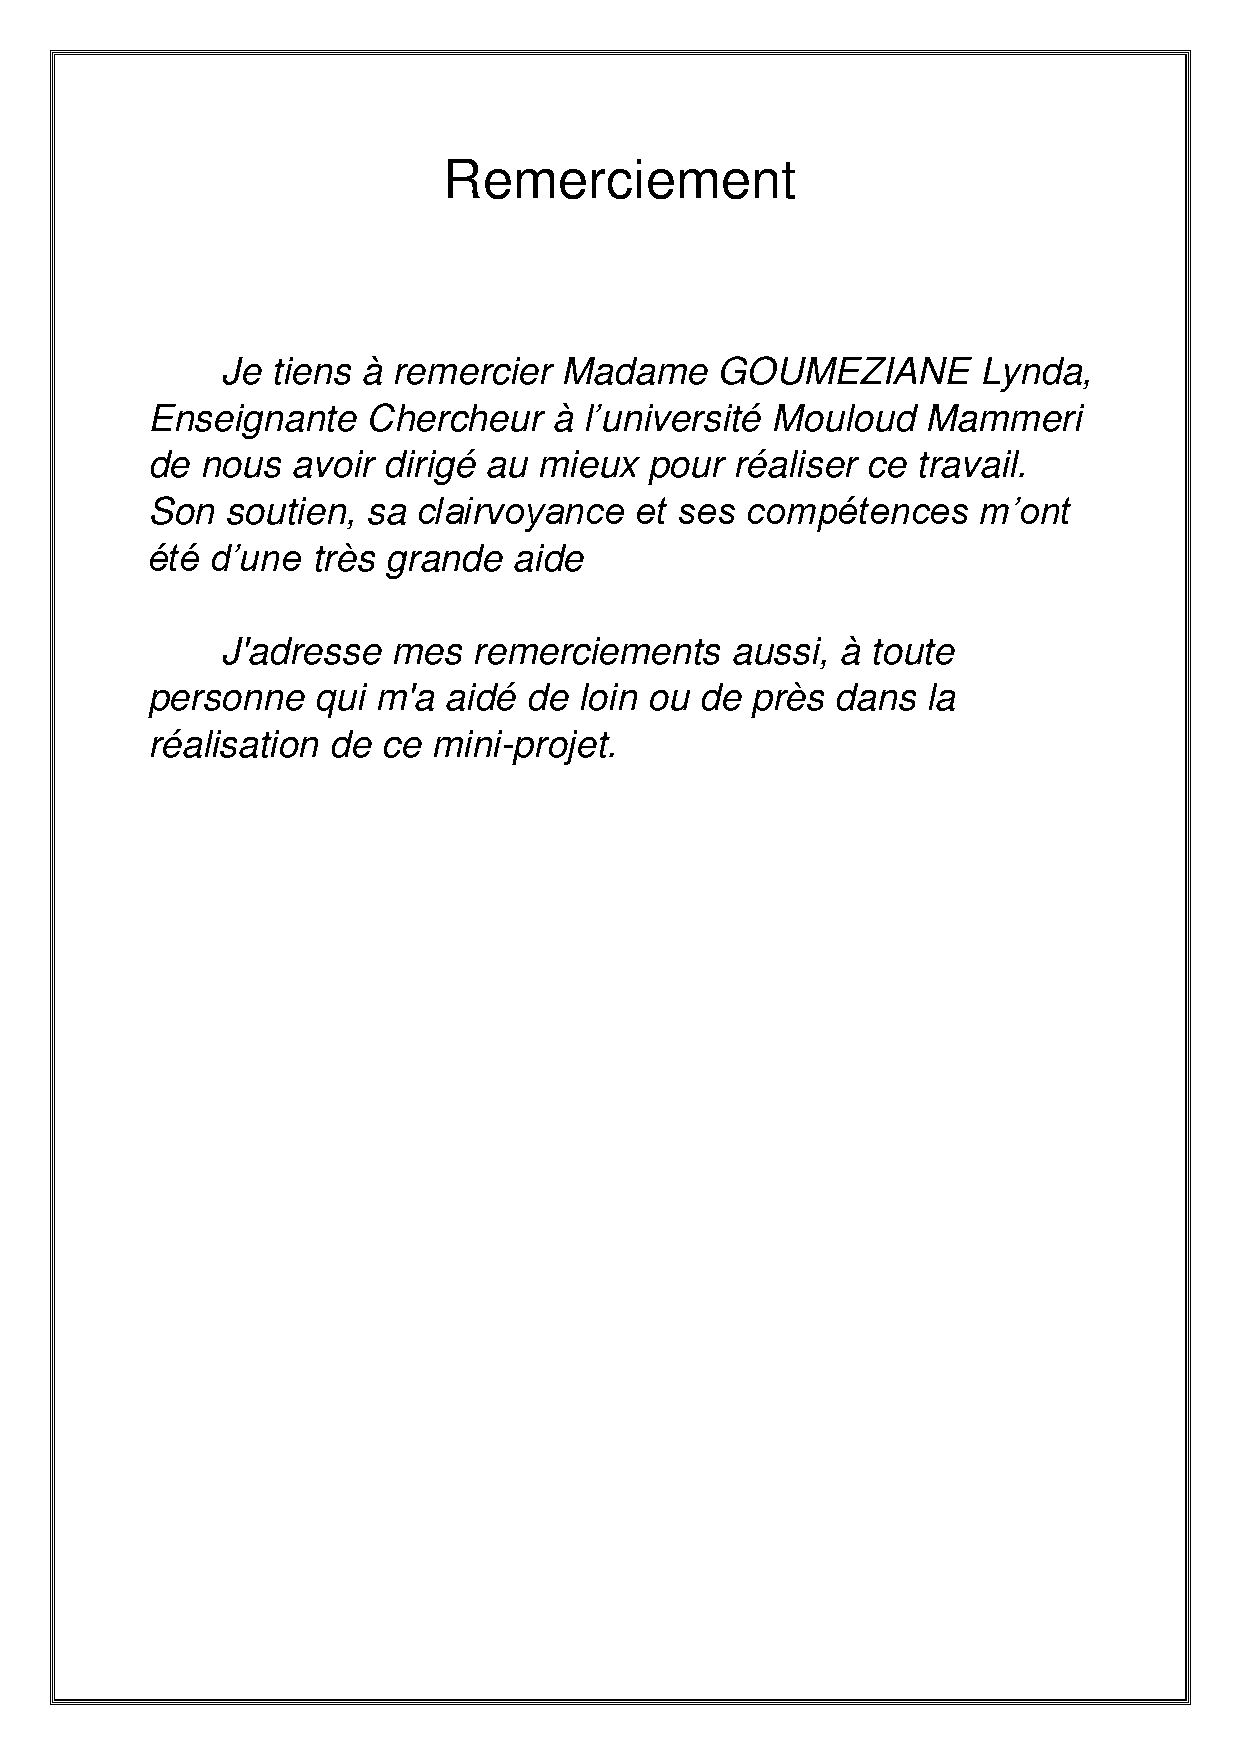
\includepdf{Remerciement-et-dedicace.pdf}
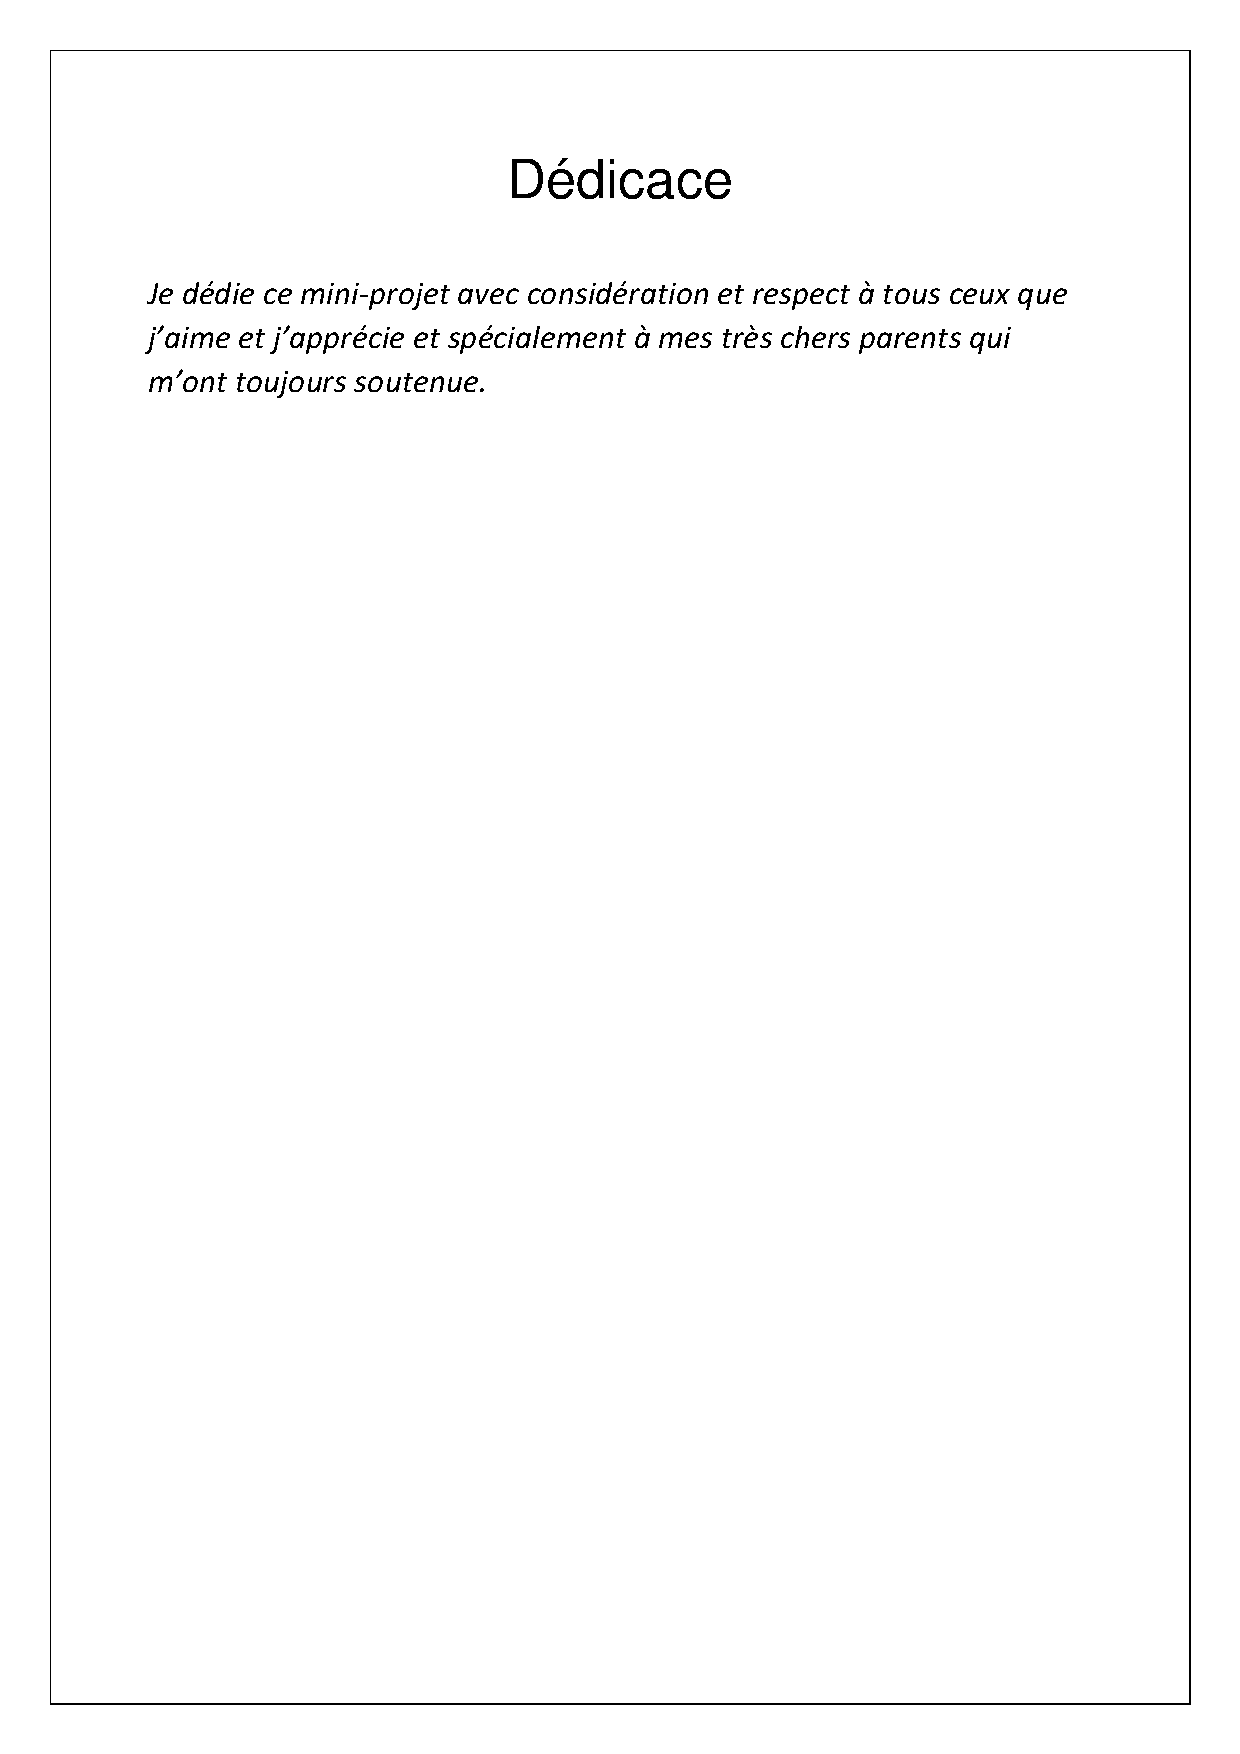
\includepdf{ded.pdf}
%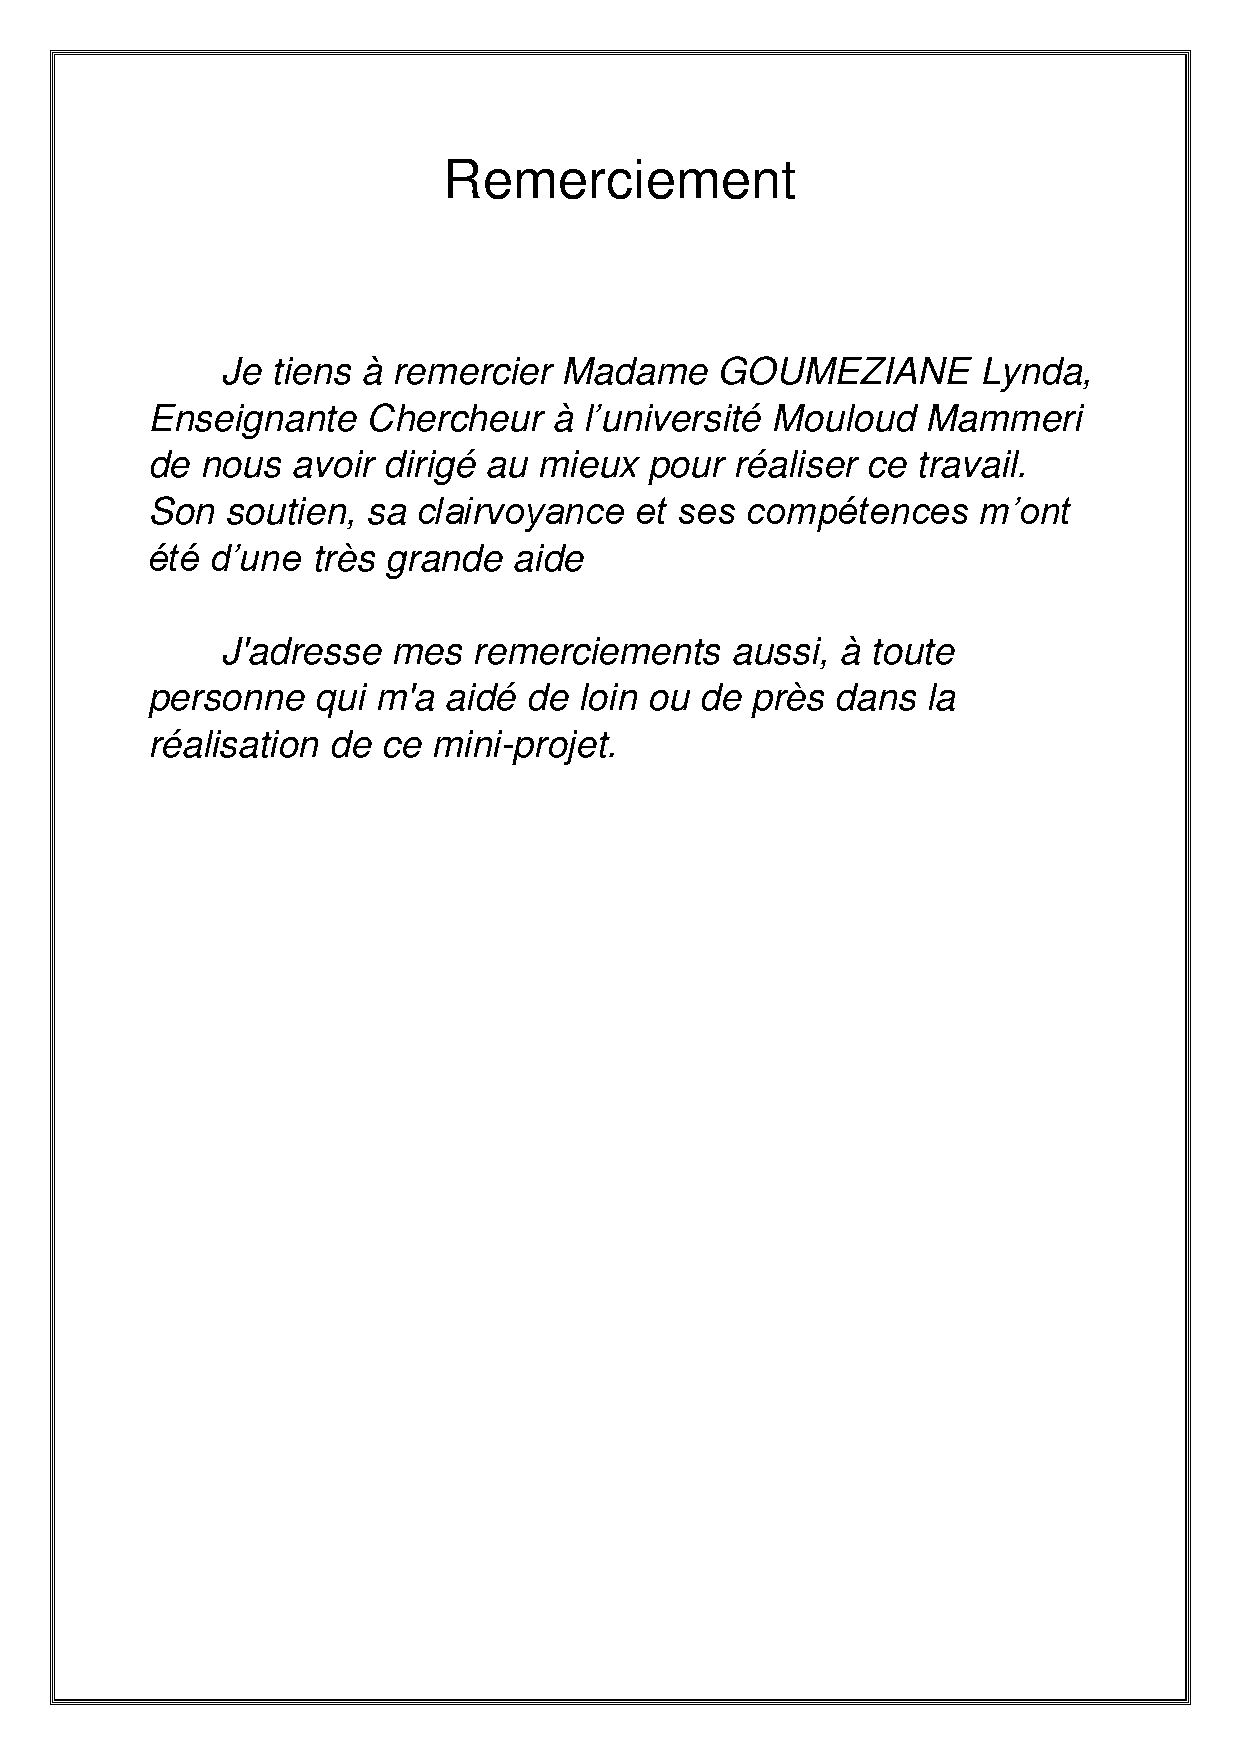
\includepdf[page=3]{Remerciement-et-dedicace.pdf}

%--------------Les diff�rentes tables--------------------------%
\renewcommand{\thepage}{}
\tableofcontents     % G�n�rer la table des mati�res automatiquement.

\phantomsection\large\addcontentsline{toc}{chapter}{Figures}\listoffigures
%G�n�rer la liste des figures automatiquement.
\renewcommand{\thepage}{}
\phantomsection\large\addcontentsline{toc}{chapter}{Tableaux}\listoftables % %G�n�rer la liste des tableaux automatiquement.
\renewcommand{\thepage}{}
%\maketitle % pour afficher le titre du memoire

\renewcommand{\thepage}{\arabic{page}} % Choisir le type de num�rotation utilis�e.(on peut utiliser aussi roman)

\setcounter{page}{+0}
\phantomsection\large\addcontentsline{toc}{chapter}{Introduction g�n�rale}  % Pour introduire l'introduction � la table de mati�re.
\chapter*{\bfseries Introduction g�n�rale} %Nom du chapitre
 � Seuls ceux qui ont v�cu dans une caverne ces dix derni�res ann�es ont pu ignorer
L�incroyable r�volution de l�apprentissage automatique � \cite{RN4}


 \paragraph{}
L�apprentissage automatique est un champs d��tude qui est devenu aussi vite populaire. Depuis, le mode a connu de grandes �volutions en terme d�avanc�es technologique, de centaines d�applications intelligentes ont vu le jour, tels que les assistants vocaux intelligents, le moyen de s�authentifier par empreinte digitale ou par reconnaissance faciale ou encore La traduction automatique.
 \paragraph{}
Tout au d�but de la cr�ation des applications intelligentes, les d�veloppeurs ont cherch� � les perfectionner et cela en r�coltant d�abord un grand nombre de donn�es puis en construire des jeux de donn�es avec lesquelles ils pourront tester et entra�ner l�application afin qu�elle puisse en tirer le vrai du faux et appliquer le concept pour toutes autres donn�e inconnue, de cette fa�on l�application apprend ce qu�elle � faire � force de tester un grand nombre d�informations et c�est cette �tude qu�on appelle l�apprentissage automatique.
 \paragraph{}
\cite{RN4}Que l�on ne soit qu�un simple utilisateur d�internet pour quelques minutes n�emp�che qu�une horde de syst�mes d�apprentissage automatique s�activent faisant des sites qu�on visite l�un des moyens qui permette d�analyser notre personnalit� pour nous proposer des produits id�als, attirer notre attention ou encore analyser nos comportements pour s�assurer que l�on est pas un fraudeur.
 \paragraph{}
   L'apprentissage automatique apprend gr�ce � nous, elle utilise nos informations que les collecteur de donn�e ou les data setter r�coltent, et cela � travers nos acc�s aux sites internet mais le nombre de ces donn�es doit �tre tr�s grand, afin de permettre � la machine d��tudier plusieurs cas et parfois m�me distinguer des anomalies, comme par exemple traiter des donn�es concernant le type de sang des �tres humain et en tirer une nouvelle sorte qu�elle isolera et quelle  consid�rera ainsi comme une anomalie.
 \paragraph{}
\cite{RN2}L�apprentissage automatique � �volu� par �tape de plus en plus complexe, Le premier mod�le d'apprentissage automatique impliquait des d�cisions bas�es sur des r�gles d�un niveau simple, ces r�gles sont sous forme d�algorithmes qui comprenait en elle-m�me des donn�es ce qui implique que toutes les options possibles seront cod�es dans le mod�le par un expert en la mati�re. Cette structure a �t� mise en �uvre dans la majorit� des applications d�velopp�es depuis l'apparition des premiers langages de programmation c�est-�-dire depuis \textcolor[rgb]{0.00,0.50,0.00}{1950}.
 \paragraph{}
 Au cours du deuxi�me mod�le, les caract�ristiques probabilistes des donn�es ont �t� faites afin qu�elles prennent des d�cisions, c�est comme si qu�elle avait un mot � dire et ceci r�gle en mieux les diff�rents probl�mes du monde r�el.
   \paragraph{}
   Le troisi�me mod�le de complexit� est d�utiliser des caract�ristiques qui ne se limite pas qu�� une fonction cible, car ces caract�ristiques sont g�n�r�es et d�finis au fur et � mesure de l��volution du processus de r�alisation du mod�le, autre �l�ment diff�renciateur de ce type de mod�le est qu'ils peuvent prendre en entr�e une grande vari�t� de types de donn�es, tels que la parole, les images, la vid�o, le texte, etc.
  \paragraph{}
  Le dernier mod�le de complexit� est l�intelligence artificiel incluant tous les types d�algorithmes pr�c�dents mais avec une diff�rence essentielle : les algorithmes de l�intelligence artificielle sont capables d�appliquer les connaissances apprises pour r�soudre des t�ches qui n'avaient jamais �t� envisag�es pendant la r�alisation du mod�le, les types de donn�es avec lesquels cet algorithme travaille sont encore plus g�n�riques que les types de donn�es pris en charge par l�intelligence artificielle, ils devraient �tre capables, par d�finition, de transf�rer les capacit�s de r�solution de probl�mes d'un type de donn�es � un autre, sans qu'il soit n�cessaire d'effectuer un apprentissage complet, De cette fa�on, des algorithmes peuvent �tre d�velopper pour d�tecter des objets dans des images, le mod�le pourrait aussi avoir la connaissance pour d�tecter des images en couleur.

  \paragraph{}
Ce travail consiste donc � donner une id�e g�n�rale sur certain concept de l�apprentissage automatique. Pour arriver � cela, le travail suivant est structur� en 2 chapitres :

     \begin{itemize}
                    \item \textcolor[rgb]{0.00,1.00,0.00}{Chapitre 1 :} est une introduction � l�apprentissage automatique.
                    \item \textcolor[rgb]{0.00,1.00,0.00}{Chapitre 2 :} est une analyse d�un des probl�mes de l�apprentissage automatique.

     \end{itemize}

Et nous terminerons ce travail par une conclusion g�n�rale.














\large \setcounter{chapter}{+0} \pagestyle{plain} % ou plain ou empty ou headings.
\chapter{\bfseries introduction � l�apprentissage automatique} %Nom du chapitre
\section{Historique de l'apprentissage automatique }
Avant de parler de notre th�matique, nous allons revenir sur son histoire.
 \paragraph{}
L�id�e de l�apprentissage automatique est due � \textbf{Alan Turing} et a son concept de la machine universelle en \textcolor[rgb]{0.00,0.50,0.00}{1963}, il posa des bases de l�apprentissage automatique en \textcolor[rgb]{0.00,0.50,0.00}{1950}. En \textcolor[rgb]{0.00,0.50,0.00}{1943}, le neurophysiologiste \textbf{Warren McCulloch} et le math�maticien \textbf{Walter Pitts} publient un article d�crivant le fonctionnement de neurones en les repr�sentant � l'aide de circuits �lectriques.
 \paragraph{}
\textbf{Arthur Samuel}, informaticien am�ricain pionnier dans le secteur de l'intelligence artificielle, est le premier � faire usage de l'expression  apprentissage automatique en \textcolor[rgb]{0.00,0.50,0.00}{1959} � la suite de la cr�ation de son programme pour \textbf{IBM} en \textcolor[rgb]{0.00,0.50,0.00}{1952}. Le programme jouait au Jeu de Dames et s'am�liorait en jouant. � terme, il parvint � battre le 4$^{\hbox{\tiny{�me}}}$ meilleur joueur des �tats-Unis.
 \paragraph{}
Durant les ann�es suivantes, les applications de l'apprentissage automatique m�diatis�es se succ�dent bien plus rapidement qu'auparavant.
 \paragraph{}
En \textcolor[rgb]{0.00,0.50,0.00}{2012}, un r�seau neuronal d�velopp� par \textcolor[rgb]{0.00,0.50,0.00}{Google} parvient � reconna�tre des visages humains ainsi que des chats dans des vid�os YouTube
 \paragraph{}
En \textcolor[rgb]{0.00,0.50,0.00}{2014}, \textcolor[rgb]{0.00,1.00,0.00}{64} ans apr�s la pr�diction d'\textbf{Alan Turing}, le dialogueur \textbf{Eugene Goostman} est le premier � r�ussir le test de Turing en parvenant � convaincre \textcolor[rgb]{0.00,1.00,0.00}{33 \%} des juges humains au bout de cinq minutes de conversation qu'il est non pas un ordinateur, mais un gar�on ukrainien de \textcolor[rgb]{0.00,1.00,0.00}{13} ans
 \paragraph{}
En \textcolor[rgb]{0.00,0.50,0.00}{2015}, une nouvelle �tape importante est atteinte lorsque l'ordinateur\textcolor[rgb]{0.00,0.50,0.00}{ � AlphaGo �} de \textcolor[rgb]{0.00,0.50,0.00}{Google} gagne contre un des meilleurs joueurs au jeu de Go, jeu de plateau consid�r� comme le plus dur du monde
 \paragraph{}
En \textcolor[rgb]{0.00,0.50,0.00}{2016}, un syst�me d'intelligence artificielle � base d'apprentissage automatique nomm� \textcolor[rgb]{0.00,0.50,0.00}{LipNet} parvient � lire sur les l�vres avec un grand taux de succ�s

\section{D�finition: (source:\cite{RN2})}
L'apprentissage automatique est une branche d'�tude dans laquelle un mod�le peut apprendre automatiquement � partir des exp�riences bas�es sur des donn�es sans �tre exclusivement mod�lis� comme dans les mod�les statistiques. Au fil du temps et avec davantage de donn�es, les pr�dictions du mod�le s'am�lioreront.
 \paragraph{}
\begin{figure}[h!]
\centering
  % Requires \usepackage{graphicx}
  
\includegraphics[width=8cm]{aa.jpg}\\
  \caption{du cerveau humain a la machine}\label{}
\end{figure}

\section{Pourquoi utiliser l'apprentissage automatique ? }
L'apprentissage automatique peut �tre utilis� pour r�soudre des probl�mes que nous ne savons pas comment r�soudre, ou bien des probl�mes qu�on sait r�soudre mais sans forc�ment savoir comment le formaliser en un algorithme de r�solution, ou que nous savons comment r�soudre, mais la proc�dure demande trop de ressources informatiques (par exemple pour la pr�diction d'interaction
Parmi les grosses mol�cules).
 \paragraph{}
Par cons�quent, utilisez le Machine Learning lorsque les donn�es sont riches,
Mais les connaissances ne sont pas facilement disponibles ou qu�elles sont sous-d�velopp�es.

L'apprentissage automatique peut �galement aider les humains � apprendre : les mod�les cr��s par des algorithmes d'apprentissage peuvent r�v�ler l'importance relative de certaines informations, ou comment elles interagissent pour r�soudre des probl�mes sp�cifiques.

\section{Probl�matique:}
L�apprentissage automatique rencontre le probl�me dit apprentissage supervis�, il s�agit des difficult�s � r�soudre des probl�mes de classification, c�est-�-dire qu�apr�s l'entra�nement d�un mod�le il est difficile de minimiser les erreurs ce qui fait qu�on est oblig� de se contenter des r�sultats qui sont peu satisfiable et qui peuvent m�me ne donner aucun r�sultat.

\section{Propositions et solutions :}
Faire recours � des algorithmes performants permettant de r�soudre des probl�mes de classification

\section{Conclusion :}
Dans ce chapitre, une vue globale de l�apprentissage automatique a �t� donn�e, la compr�hension de � quand � est apparu cette �tude a �t� mis en �vidence � travers une pr�sentation d�un historique, Ensuite la th�matique a �t� d�finit. Puis une probl�matique a �t� pos�e et afin de rem�dier � cela, une suggestion de solution est propos�e. Dans le deuxi�me chapitre, le probl�me pos� de l�apprentissage automatique sera au mieux expliqu� afin d�en aboutir � une solution.

%\subsection{D�finition}

\large  \pagestyle{plain} % ou plain ou empty ou headings.
\chapter{\bfseries Type de probl�me de l'Apprentissage Automatique  } %Nom du chapitre
%%%%%%%%%%%%%%%%%%%%%%%%%%%%%%%%%%%%%%%%%%%%%%%%%%%%%%%%%%%%%%%%%%%%%%%%%%%%%%%%%%%%%%%%%%%
%%%%%%%%%%%%%%%%%%%%%%%%%%%%%%%%%%%%%%%%%%%%%%%%%%%%%%%%%%%%%%%%%%%%%%%%%%%%%%%%%%%%%%%%%%%
\section{Apprentissage supervis�}

\subsection{D�finition (source:\cite{RN6})}
\begin{figure}[h!]
\centering
  % Requires \usepackage{graphicx}
  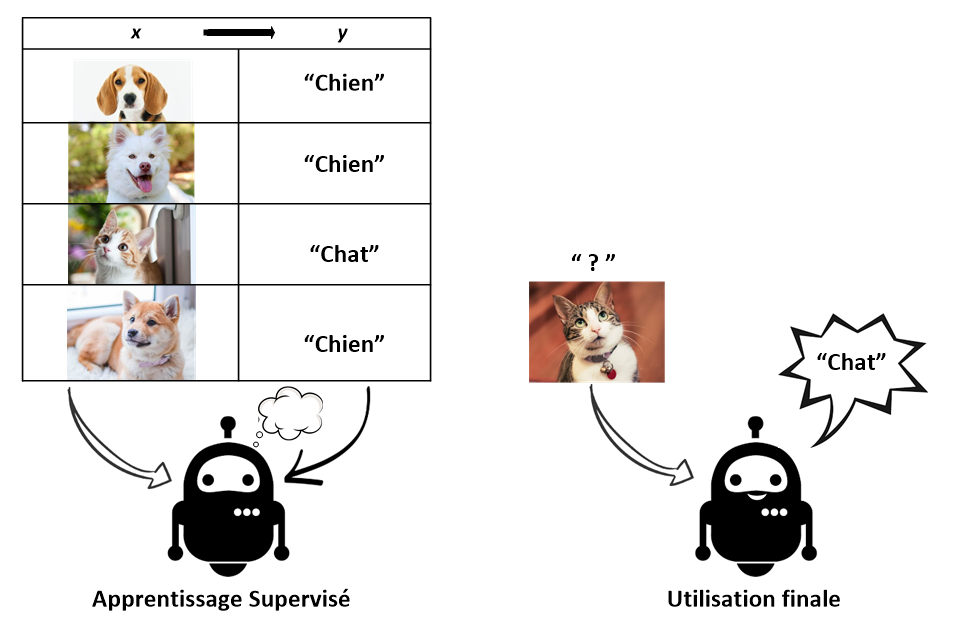
\includegraphics[width=17cm]{sup.png}\\
  \caption{Apprentissage Supervis� }\label{fig:f10}
\end{figure}
L'apprentissage supervis� n�cessite l'intervention de l'�tre humain (souvent un expert) pour sp�cifier � l'algorithme les r�sultats qu'il doit produire. L'apprentissage supervis� n�cessite que les sorties possibles de l'algorithme soient d�j� connues et que les donn�es utilis�es pour entra�ner l'algorithme sont d�j� �tiquet�s avec les bonnes r�ponses. Par cons�quent, les donn�es d'entra�nement doivent �tre �tiquet�s/class�s � l'avance en plus des caract�ristiques d'identification.
\paragraph{}


Certaines des approches utilis�es pour l'apprentissage automatique supervis� comprennent La classification et la regression .



\section{Classification }

La classification est le processus de recherche d�un mod�le (ou d�une fonction) qui d�crit et distingue des classes de donn�es ou des concepts. Le mod�le est d�riv� de l�analyse d�un ensemble de donn�es d�apprentissage (c�est-�-dire des objets de donn�es pour lesquels les �tiquettes de classe sont connues). Le mod�le est utilis� pour pr�dire l��tiquette de classe des objets pour lesquels l��tiquette de la classe est inconnue.
Le mod�le d�riv� peut �tre repr�sent� sous diff�rents formats, telles que les r�gles de classification (c�est-�-dire les r�gles Si-Alors), r�seaux de neurones, etc.

 Exemple :
un client donn� nous quittera-t-il pour un concurrent ? Est-ce qu�un patient donn� � une maladie ?
Les principaux algorithmes de classification, sont :\cite{RN5}

  \begin{itemize}
                    \item \textbf{{Algorithmes d�arbre de d�cision :}} Un arbre de d�cision construit une structure de type arbre de solutions possibles � un probl�me bas� sur certaines contraintes.
Ils sont ainsi nomm�s, car ils commencent par une simple d�cision ou racine, qui se d�compose ensuite en un certain nombre de branches jusqu�� ce qu�une d�cision ou une pr�diction soit faite, formant un arbre. Ils sont favoris�s pour leurs capacit�s � formaliser le probl�me et � fournir des solutions plus rapides et plus pr�cises compar�es � d�autres algorithmes.

Les algorithmes les plus connus sont : Arbre de classification et de r�gression
(CART), It�ratif dichotomiseur 3 (ID3), Souche de d�cision,
Arbres d�cisionnels conditionnels, etc.
\paragraph{}
                    \item \textbf{{Algorithmes bay�siens :}} est Un groupe d�algorithmes d�apprentissage automatique supervis� qui utilise le th�or�me de Bayes pour r�soudre les probl�mes de classification.
On peut citer parmi les algorithmes : Estimateurs � une d�pendance en moyenne
(AODE), Bayesian Belief Network (BBN), etc.
\paragraph{}
\item  \textbf{{k- plus proche voisin :}}
un algorithme d'apprentissage automatique supervis� qui fonctionne comme suit :

\subitem L'algorithme de classification KNN cherche � classer de nouveaux exemples de donn�es (ou d'objets), sur la base de donn�es pr�c�dentes (saisies lors de l'apprentissage).
\subitem  Chaque objet est repr�sent� par des attributs, et la comparaison de ces attributs est suffisante pour d�terminer la similitude entre deux objets.

\subitem  Plus la diff�rence entre deux objets est petite, plus ils sont similaires.

\subitem  La similitude entre l'objet A avec les attributs {a1, a2, ..., an} et l'objet B avec les attributs {b1, b2, ..., bn} peut �tre calcul�e en utilisant la distance euclidienne :
\paragraph{}
$$d\left( p,q\right)= \sqrt {\sum _{i=1}^{n}  \left( q_{i}-p_{i}\right)^2 }$$

     \end{itemize}

\paragraph{}
On constate donc que des algorithmes ont �t� d�velopper et mis en point afin de r�gler les probl�mes de classification.
Plusieurs autres algorithmes peuvent aussi r�gler ce type de probl�me.
Le tableau ci-dessous nous montre en vue plus globales ces algorithmes:



\begin{table}[h!]
\begin{Large}
\begin{center}
\begin{tabular}{l|c|c}
~~ & $Algorithme$ & $En~~anglais$ \\ \hline
1 &  R�gression logistique & Logistic regression \\ \hline
2 & K-plus proches voisins & K-nearest neighbour (KNN)\\ \hline
3 & Machines � vecteurs de support& Support vector machines (SVM) \\ \hline
4 &Classification na�ve bay�sienne & Naive Bayes classification (NB)\\ \hline
5 & Arbres de d�cision& Decision trees (DT)\\ \hline
6 &For�ts al�atoires & Random forest (RF) \\ \hline
7 & R�seaux de neurones & Neural Networks (NN) \\
\end{tabular}
\end{center}
\caption{Tableau d'algorithmes de classification }
\end{Large}
\end{table}



\section{autres m�thodes d�apprentissage:}
\subsection{r�seaux de neurones: }\cite{RN5}


Les r�seaux de neurones sont une mod�lisation math�matique simple, utilisant des entit�s �l�mentaires (neurones) poss�dant une sortie et plusieurs entr�es. Le neurone somme ses entr�es et applique une fonction d'activation pour g�n�rer sa sortie. Un r�seau de neurone utilise de milliers, millions voir milliards de ces entit�s, connect�es les unes aux autres par couche de neurones.
Si le lecteur peut retrouver dans la terminologie propre � ce domaine des mots tir�s de la biologie, il ne faut cependant pas penser que le but des r�seaux de neurones g�n�ralement utilis�s est de fournir une mod�lisation du fonctionnement du cerveau il s'agit plut�t d'une mod�lisation grossi�re, permettant d'approximer n'importe quelle fonction non-lin�aire (ce sont des approximates universels).
Certains r�seaux de neurones sont tout de m�me utilis�s pour leur plausibilit� : c'est notamment le cas des spiking neural networks, utilisant une mod�lisation du fonctionnement �lectrique des neurones pour r�soudre des t�ches.
\paragraph{}
Il ne s'agit cependant pas l� des mod�les les plus utilis�s. Les r�seaux de neurones utilis�s couramment sont assez semblable � celui pr�sent� sur la figure \ref{fig:f1} Ils se composent d'une couche d'entr�e, une ou plusieurs couches cach�es et une couche de sortie.
\paragraph{}
Les poids reliant la sortie d'une couche aux entr�es de la couche suivante sont des param�tres qui sont optimis�s lors d'une phase appel�e "apprentissage" (ou training). Durant cette phase, on utilise g�n�ralement un jeu d'entr�es/sorties. En comparant la sortie attendue avec la sortie de notre mod�le, on est capable de modifier les poids reliant les couches de mani�re � faire converger, tout au long de l'apprentissage, la sortie du mod�le vers la sortie attendue.
La r�elle force des r�seaux de neurones r�side dans leur capacit� � g�n�raliser. Si l'apprentissage est stopp� assez t�t (early stop, permettant d'�viter l'overfitting, le sur-apprentissage), le mod�le est capable de :
\paragraph{}
-R�pondre presque correctement lorsque l'on lui passe une entr�e du jeu de donn�es.
-R�pondre presque correctement lorsque l'on lui passe une entr�e qui ne fait pas partie du jeu de donn�es.
\paragraph{}
Cela veut dire que ces r�seaux peuvent, � partir d'une faible quantit� de donn�es caract�risant un ph�nom�ne, d'extraire les concepts principaux de mani�re � g�n�raliser et mod�liser ce ph�nom�ne.

\begin{figure}[h!]
\centering
  % Requires \usepackage{graphicx}
  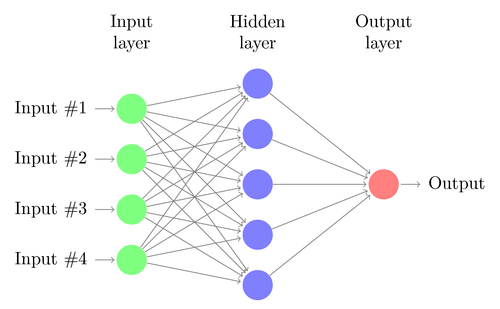
\includegraphics[width=8cm]{neural-network.png}\\
  \caption{Un r�seau de neurones � trois couches successives}\label{fig:f1}
\end{figure}

\paragraph{}
Un des hyper param�tres important des r�seaux de neurones est la capacit� du r�seau, qui d�pend du nombre de neurones pr�sent. La capacit� influe sur la facult� d'un r�seau � approximer une fonction pr�cis�ment.
On peut intuitivement se dire que plus la capacit� sera grande, plus le r�seau pourra approximer une fonction pr�cis�ment. Ceci est totalement faux : la capacit� d'un r�seau de neurones doit correspondre avec la complexit� de la fonction, comme on peut le constater en figure \ref{fig:f2}


\begin{figure}[h!]
\centering
  % Requires \usepackage{graphicx}
  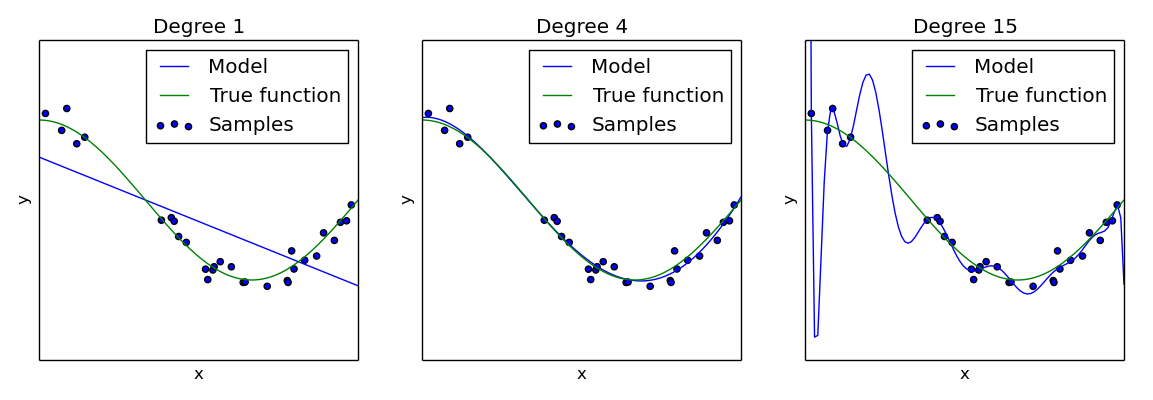
\includegraphics[width=15cm]{plot.png}\\
  \caption{De gauche � droite : une capacit� trop faible, correcte et trop �lev�e pour la t�che.}\label{fig:f2}
\end{figure}

 \paragraph{}
                    Cette id�e d'utiliser des d'unit�s g�n�riques performant une simple op�ration dans
                    des r�seaux pour g�n�rer ou appr�hender des comportements complexes date de 1943
                    (McCulloch et Pitts). Ceci a connu un fort essor jusqu'aux ann�es 1980 (avec la
                    cr�ation du n�ocognitron de Kunihiko Fukushima, r�seau de neurones proche des
                    architectures modernes).

                \paragraph{}
                    On se rend alors vite compte du probl�me de sur-apprentissage, et de la
                    difficult� de r�aliser des r�seaux de neurones de tr�s grande capacit�.
                    Arrive alors une stagnation dans le domaine, malgr� quelques avanc�es
                    comme la cr�ation r�seaux de neurones conventionnels par Yann Le Cun
                    (aujourd'hui directeur du groupe de recherche en IA de Facebook).
                    C'est en 2012 que, sur les travaux de Le Cun,  A. Krizhevsky, I. Sutskever, et G. E. Hinton
                    publient "Imagenet classification with deep convolutional neural networks".

                \paragraph{}
                    Dans cette publication, les auteurs r�ussissent � cr�er et entra�ner un r�seau
                    de neurones dit \textit{profond} (d'une grande capacit�, d'o� le \textit{deep learning})
                    pour classifier des images d'un �norme jeu de donn�es avec une pr�cision
                    jamais �gal�e.

                \paragraph{}
                    Depuis lors, nous connaissons un essor consid�rable de l'intelligence
                    artificielle, notamment chez les g�ants de l'Internet. C'est gr�ce � cela
                    que Facebook est capable de proposer des identifications automatiques sur
                    des photos, ou que Google Assistant est capable de nous comprendre et
                    d'interpr�ter nos questions.

                \paragraph{}
                    Ces nouvelles innovations sont fortement prometteuses pour la robotique,
                    dans le domaine de la vision ou de la planification de trajectoire,
                    mais aussi pour compenser les erreurs de mod�les, lorsque que l'on transfert
                    un programme fonctionnant en simulation sur un robot r�el.
\section{De l'apprentissage automatique vers l'intelligence artificiel (source:\cite{RN3})}
Les m�thodes d'apprentissage automatique ont �volu� rapidement au cours des derni�res ann�es, mais une tendance plus importante a commenc� il y a environ dix ans. Plus pr�cis�ment, le domaine de la science des donn�es a �merg� et nous sommes pass�s des statisticiens aux ing�nieurs informatiques et aux algorithmes \ref{fig:f10}
\begin{figure}[h!]
\centering
  % Requires \usepackage{graphicx}
  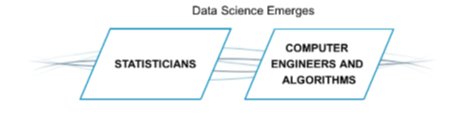
\includegraphics[width=15cm]{10.png}\\
  \caption{L'�volution des statisticiens vers les ing�nieurs informatique et algorithmes}\label{fig:f10}
\end{figure}

La statistique classique �tait le domaine des math�matiques et des distributions normales.
\paragraph{}
La science moderne des donn�es est infiniment flexible sur la m�thode ou les propri�t�s, tant qu'elle met en �vidence un r�sultat pr�visible. L'approche classique impliquait une mani�re unique de r�soudre un probl�me. Mais les nouvelles approches varient radicalement, avec de multiples voies de solution.

\section{Conclusion}

Nous venons de voir un des probl�me de l'apprentissage automatique, a savoir le probl�me de classification, en premier lieu on a d�finit l'apprentissage supervis�, puis la classification et nous avons aussi s'approfondir sur les m�thodes d'apprentissage disponible comme les reseaux de neurones qui figurait dans la liste des algorithmes r�glant le probl�me de classification et en terminant, nous somme allez au del� de l'apprentissage automatique c'est-a-dire vers l'intelligence artificielle qui lui, englobe ce champ d'�tude.





\phantomsection\large\addcontentsline{toc}{chapter}{Conclusion g�n�rale}  % Pour introduire l'introduction � la table de mati�re.
\chapter*{\bfseries Conclusion g�n�rale.} 
Ce mini-projet, a pour objectif de nous introduire � l�apprentissage automatique en s�inspirant de certains auteurs qui ont �tudier le domaine de l�intelligence artificiel, permettant d�une part aux lecteur d�avoir une id�e d�ensemble et d�autre part de conna�tre un des principaux types de probl�me de l�apprentissage automatique �tant le syst�me d�apprentissage supervis� �tudiant le probl�me majeur de classification gr�ce a des algorithmes mis en point par des grands chercheurs.
Nous avons r�parti notre travail en deux chapitres :
\paragraph{}
  \begin{itemize}
                    \item \textcolor[rgb]{0.00,1.00,0.00}{Chapitre 1 :} est une introduction � l�apprentissage automatique.
                    \item \textcolor[rgb]{0.00,1.00,0.00}{Chapitre 2 :} est une analyse d�un des probl�mes de l�apprentissage automatique.

     \end{itemize}
\paragraph{}
La r�alisation de ce travail a permis d�acqu�rir des connaissances dans le domaine informatique, sp�cialement, le domaine de l�intelligence artificielle et plus pr�cis�ment, le champs d��tude � l�apprentissage automatique �.
\paragraph{}
En utilisant un bagage acquis auparavant � travers les cours d�intelligence artificielle, et en faisant des recherches bibliographiques nous somme arriver � conclure que la classification est finalement un probl�me r�glable � l�aide d�algorithmes con�u sp�cialement pour cela mais qui demande beaucoup de recherche afin de r�colter beaucoup d�informations n�cessaire � cette solution.
\paragraph{}
Nous esp�rons revoir ce probl�mes de l�apprentissage supervis� et mettre au point un des algorithmes cit� et ceci dans le but de comprendre au mieux comment les probl�mes sont r�gl�s.


%%%%%%%%%%%%%%%%%%%%%%%%%%%%%%%%%%%%%%%%%%%%%%%%%%%%%%%%%%%%%%%%%%%%%
%%%%%%  Pour cr�er une bibiliographie apartir d'un fichier    %%%%%%%
%%%%%%  bibtex qui organisera automatiquement cette derniere  %%%%%%%
%%%%%%%%%%%%%%%%%%%%%%%%%%%%%%%%%%%%%%%%%%%%%%%%%%%%%%%%%%%%%%%%%%%%%

\newpage
\bibliographystyle{plain}\markboth{Bibliographie}{}
\nocite{*}\sloppy\pagestyle{empty}\phantomsection
\addcontentsline{toc}{chapter}{Bibliographie} % Pour ajouter la bibliographie � la table de mati�re.
\bibliography{biblio}

%%%%%%%%%%%%%%%%%%%%%%%%%%%%%%%%%%%%%%%%%%%%%%%%%%%%%%%%%%%%%%%%%%%%%%%%%%%%%%%%%%%%%%%
\end{document} 